%!TEX root = ../thesis.tex
%*******************************************************************************
%*********************************** First Chapter *****************************
%*******************************************************************************

\chapter{Total Monte Carlo propagation of nuclear data uncertainties to nuclear fusion engineering parameters} %Title of first chapter
\label{chap:tmc}

\ifpdf
    \graphicspath{{Chapter1/Figs/Raster/}{Chapter1/Figs/PDF/}{Chapter1/Figs/}}
\else
    \graphicspath{{Chapter1/Figs/Vector/}{Chapter1/Figs/}}
\fi

%\nomenclature[g-pi]{$\pi$}{ $\simeq 3.14\ldots$}

\section{Outline}

%%%% OUTLINE GOES HERE

%********************************** %First Section  **************************************
\section{Introduction}

\label{introduction}
A handful of different fusion fuels were discussed in the opening chapter. The cross-section and Q-value of the D-T reaction make a burning plasma the most easily realisable. However, sustainably liberating energy from the D-T fusion reaction requires a reliable supply of tritium fuel. Given tritium is not naturally occuring, with a $t_{\frac{1}{2}}=12.3y$ \nomenclature[a]{$t_{\frac{1}{2}}$}{Half-life} it must be artificially produced. It is worth considering whether this could be outsourced to a third party given the complexity of `grow-your-own'. The HWR reactors of Canada, Romania and the Republic of Korea produce small amounts of tritium each year, but significantly less than is required for the operation of a fusion power plant. In fact, these facilities will struggle to provide the relatively small amounts of tritium necessary for the start-up of a device \cite{Kovari2018}. Given that, future plant must be tritium self-sufficient. Neutrons will initiate tritium producing reactions in $^{6,7}$Li contained within a blanket. Depending on the blanket design, the tritium will either be purged or natually `outgas' before filtration and storage. 

The ratio of tritium produced to tritium consumed is known as the Tritium Breeding Ratio (TBR). An equation for the TBR is given as equation~\ref{eq:tbr} where $T_{prod}$ is tritons produced in the blanket, $T_{cons}$ tritons consumed in the plasma, $N_{s}$ the number density of each nuclide, $\sigma_{r}$ the r\textsuperscript{th} tritium producing reaction cross-section for that nuclide and $\phi(E)$ the neutron flux as a function of energy. 

\begin{equation}
  \label{eq:tbr}
  \mathrm{TBR} = \frac{T_{prod}}{T_{cons}} = \frac{\sum_{s=1}^{S} N_{s}}{T_{cons}} \int_{0}^{\infty} \phi(E) \sum_{r=1}^{R} \sigma_{r}(E) dE
\end{equation}

Two reactions in lithium produce the majority of tritium in the blanket and are shown below. Both naturally occuring lithium isotopes have an anomolously low nuclear binding energy per nucleon. This is why \textsuperscript{6}Li can exothermically fission despite being such a light nuclide. With the reaction being exothermic, its likelihood gains with decreasing interaction energy, meaning neutrons of all energies may potentially contribute to tritium production. Conversely, the tritium producing \textsuperscript{7}Li reaction is endothermic, with a threshold interaction energy of approximately 2.47 MeV. Natural lithium is $\approx 7.5\%$ \textsuperscript{6}Li with the remainder \textsuperscript{7}Li. Fusion breeding blankets will need their \textsuperscript{6}Li to be isotopically enriched to achieve an acceptable TBR.

\begin{equation}
\begin{split}
  ^{6}\mathrm{Li} + \mathrm{n} & \rightarrow \alpha + \mathrm{T} + 4.8\mathrm{MeV} \\
  ^{7}\mathrm{Li} + \mathrm{n} & \rightarrow \alpha + \mathrm{T} + \mathrm{n} - 2.5\mathrm{MeV}
\end{split}
\end{equation}

There are other reactions for creating tritons. For instance, the tritium decay product, $^{3}\mathrm{He}$ has an affinity for thermal neutrons and can be transmuted back to tritium by them. There is also a small chance of neutron capture leading to tritium production in $^{10}\mathrm{B}$.

\begin{equation}
\begin{split}
  ^{3}\mathrm{He} + \mathrm{n} & \rightarrow p + \mathrm{T} \\
  ^{10}\mathrm{B} + \mathrm{n} & \rightarrow 2\alpha + \mathrm{T}
\end{split}
\end{equation}

There also a variety of multi-step pathways which produce tritium via the creation of other intermediate nuclides. 

Within all proposed breeding systems there are a variety of tritium loss mechanisms: absorption in materials, leakage in the tritium extraction system and radioactive decay. To accommodate these losses and still retain a TBR in excess of unity, a margin, $M$ is employed: $\mathrm{TBR} = 1 + M$. There is a constraint on the maximum allowable tritium inventory at a given facility on the order of kilograms. The window of adequate tritium supply is therefore relatively narrow and TBR should be precisely known and/or adjustable to keep within this window. Unfortunately there are many sources of uncertainty within TBR calculations. These can broadly be categorised as: poor/missing nuclear data, modelling simplifications and Monte-Carlo statistical uncertainty. Nuclear data often contributes the greatest uncertainty to TBR \cite{El-Guebaly2009}. However, the effect of these uncertainties is rarely reported alongside calculated TBR values. This is in large part due to the difficulty of propagating uncertainty data through a Monte-Carlo radiation transport simulation to the uncertainty on integral quantities of interest. Any uncertainties that are propagated are generally based on a simplified uncertainty treatment that does not include full energy, emitted double-differential and channel-to-channel correlations. 
% ^^ needs cleaning up - does it flow in terms of concepts?

A sensitivity analysis of Helium Cooled Lithium Lead (HCLL) \nomenclature[z]{HCLL}{Helium Cooled Lithium Lead} type breeder blankets for the ITER Test Blanket Modules (TBM) \nomenclature[z]{TBM}{Test Blanket Module} has identified $^{6}$Li, $^{56}$Fe and the Pb cross-sections as the most important for TBR uncertainty \cite{Leichtle2011}. This chapter quantifies the TBR uncertainty introduced by Pb nuclear data on the HCLL DEMO blanket design by employing the Total Monte Carlo (TMC) \nomenclature[z]{TMC}{Total Monte Carlo} uncertainty propagation methodology.

% \begin{figure}
% %  \figuretitle{}
%   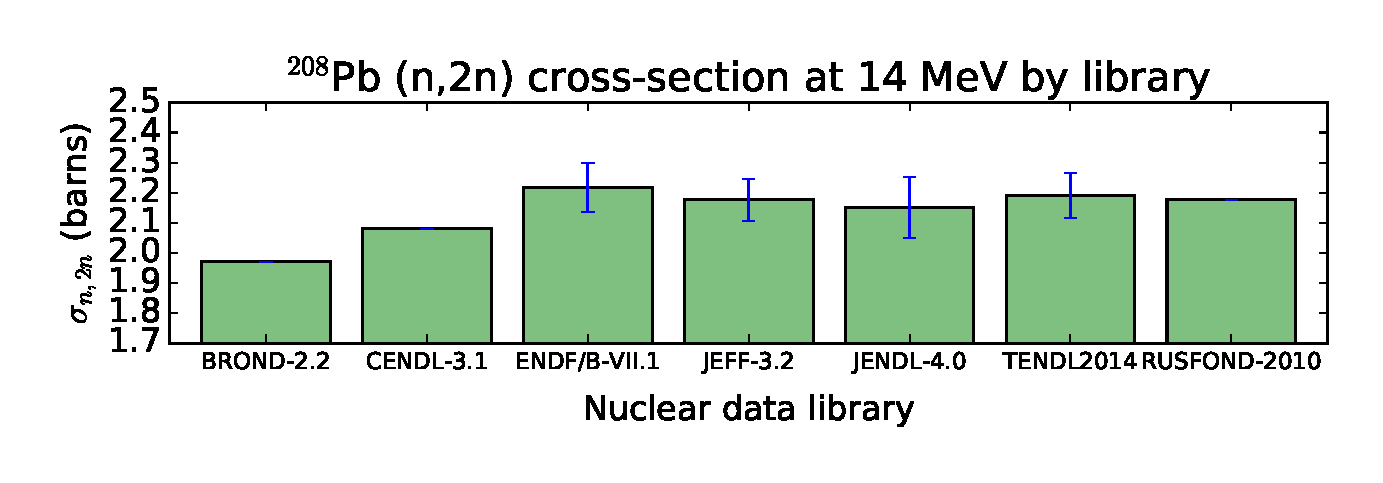
\includegraphics[width=0.47\textwidth]{pb208_n2n_by_lib}
%   \caption{$^{208}$Pb(n,2n)$^{207}$Pb cross-sections at 14MeV with their associated uncertainties for various libraries.}
%   \label{fig:lead_by_library}
% \end{figure}

% Read through section, decide on underlying topics
% Generate sub headings 
% Find papers
% Summarise and write

% HEADINGS
% Uncertainty propagation (see Michael Rising)
%   ? Conventional ?
%   Total Monte Carlo
% Uncertainty in fusion relevant nuclear data
%   Example - DT cross-section?
%   Example - Be multiplicity? O-16 scatter?
%   Example - Lead multiplicity
% END HEADINGS

\subsection{Uncertainty propagation}
% Rising pg 90, ref 83,84
The uncertainty in ND only has intrinsic interest for ND specialists. After all, these uncertainties are a result of our lack of knowledge, they are not a physical quantity. Those in the nuclear engineering field who use this data are more concerned with how `integral' quantities such as heating rates, neutron fluences, TBRs, etc. are impacted by ND uncertainties. To estimate this, one must `propagate' the uncertainty from data to integral quantities. The main approaches are pertubation theory / sensitivty analysis and sampling methods. Perturbatory approaches were developed first, with sampling methods only becoming available with the increases in computing power achieved in the 21\textsuperscript{st} century. Both methods are detailed below.
\subsubsection{Perturbation and sensitivity}
Perturbation theory is widely applied in many branches of the sciences, and generally consists of substituting an unsoluble equation for a related, soluble one plus some perturbatory series of terms. These increasing order terms have less and less impact on the result and the series is truncated at some point. 

Work on applying this approach to reactor physics problems was undertaken by Wigner on the first nuclear pile \cite{Rising2012}. A more sophisticated framework was developed by Gandini, the Generalised Perturbation Theory (GPT) \cite{Gandini1967} and subsequently into the Equivalent Generalised Perturbation Theory (EGPT) \cite{Gandini1986}. These efforts require obtaining the forward and adjoint solutions to the Boltzmann transport equation such that one can identify the magnitude of responses to any input perturbation. This means GPT and EGPT naturally lend themselves to deterministic methods for radiation transport, where full solutions to the Boltzmann equation are obtained, rather than a subsection of its phase space sampled (as in stochastic methods). This was overcome relatively recently for fission with codes like TSUNAMI-3D by Rearden, which can calculate uncertainties in $k_{\mathrm{eff}}$ with deterministic or Monte Carlo methods \cite{Rearden2004}. An alternative method, not specific to fission problems, is to couple a radiation transport code such as MCNP \cite{} with the SUSD or SUS-3D codes \cite{}. MCNP is used with perturbed cross-sections to determine how sensitive, $S$, a response parameter, $R$, is to changes, $\delta \sigma_{g}$, in a cross-section group, $\sigma_{g}$, as shown in equation~\ref{eq:sensitivity}.

\begin{equation}
  \label{eq:sensitivity}
  S = \frac{(\delta R)/R}{(\delta \sigma_{g}) / \sigma_{g}}
\end{equation}

SUSD can be used to combine processed covariance information with these sensitivity profiles to determine the uncertainty in various response parameters. Further detail on perturbation theory applied to radiation transport systems can be found in \cite{Sabouri2013}.

A disadvantage of perturbation theory methods is that they are only valid for `small' perturbiations in input quantities, which is unfortunate if some nuclear data evaluation is particularly poorly known and so of most importance to propagate. Another disadvantage is perturbation approaches may yield the variance in some integral quantity due to a varied input, but not the higher-order moments of any distribution. Hence the skewness or kurtosis cannot be known, even if the underlying distribution is non-normal.

\nomenclature[z]{GPT}{Generalised Perturbation Theory} 
\nomenclature[z]{EGPT}{Equivalent Generalised Perturbation Theory} 
\nomenclature[z]{TSUNAMI-3D}{Tools for Sensitivty and Uncertainty Analysis Methodology Implementation in three Dimensions}

\subsubsection{Total Monte Carlo}
TMC, or Total Monte Carlo, takes a different approach to perturbation theory. Rather than calculate sensitivity profiles for various minor changes to input data, here a calculation is run many times, each calculation sampling from specially prepared `random' ND libraries which encompass the distribution likely values. Assuming quality data can be generated, and computing power is not scarce, this offers several benefits. 

\subsection{Uncertainty in fusion relevant data}
  \cite{Forrest2011}
\subsubsection{Deuterium-Tritium}
\subsubsection{\textsuperscript{16}O scattering}
\subsubsection{Lead multiplicity}

Cross-section uncertainties can be represented as single values for a given energy and reaction channel. As an example, the $^{208}$Pb(n,2n)$^{207}$Pb reaction at 14MeV is shown in Table \ref{tab:lead_by_lib} for a variety of nuclear data libraries. Information on how uncertainty for a given energy affects other energies is quantified in energy covariance matrices, but these are not available for the majority of reaction channels in standard nuclear data libraries.

\begin{table}[ht]
  \footnotesize
  \centering
  \begin{tabularx}{\textwidth}{XXXX}
    \toprule
    Source & Energy [MeV] & $\sigma_{n,2n}$ [b] & $\pm\%\Delta\sigma_{n,2n}$ \\
    \midrule
    BROND 2.2 & 14.0 & 1.97 & - \\
    CENDL 3.1 & 14.0 & 2.08 & - \\
    ENDF/B-VII.1 & 14.0 & 2.22 & 8.15 \\
    JEFF 3.2 & 14.0 & 2.18 & 7.0 \\
    JENDL 4.0 & 14.0 & 2.15 & 10.1 \\
    TENDL 2015 & 14.0 & 2.19 & 7.4 \\
    RUSFOND 2010 & 14.0 & 2.18 & - \\
    EXFOR: Simakov & 14.1 & 2.38 & 5.88 \\
    EXFOR: J. Frehaut & 14.28 & 1.97 & 8.57 \\
    \bottomrule
  \end{tabularx}
  \caption{Cross-section values for the n,2n reaction channel, $\sigma_{n,2n}$ around 14 MeV for various libraries and experiments. The ENDF utility code Inter \cite{inter} was used to extract the values for each library. The two experimental results were retreived from the online EXFOR database \cite{exfor2017}. The uncertainties, $\Delta\sigma_{n,2n}$ are presented as percentages above and below the reported value.}
  \label{tab:lead_by_lib}
\end{table}

The TENDL-2015 library is a comprehensive, general-purpose nuclear data library which contains data on interactions between 7 projectiles and over 2,800 target nuclides. The library is produced by a suite of codes known as T6 and an adherance to a strict methodology of reproducability \cite{Rochman2016}. It uses the TALYS nuclear reaction code to model reactions and predict nuclear data. The inputs are fundamental parameters, including data from the RIPL-3 database \cite{RIPL3}, each with their own probability distributions that reflect their uncertainties. For the TENDL libraries, the distribution of nuclear data contained in the files with sampled input parameters can give more information on nuclear data uncertainty than is contained in a traditional evaluated nuclear data file. The shape of the distribution are captured and need not necessarily be simple Gaussian.

The Total Monte-Carlo (TMC) method utilises nuclear data generated from these sampled fundamental parameters to quantify uncertainties on integral quantities. With a given ensemble of sampled nuclear data, a radiation transport simulation is performed and an observable recorded. The process is repeated hundreds of times to produce a distribution of the observable of interest, with the uncertainty in the fundamental parameters used in the genration of self-consistent nuclear data files, propagating the fully-correlated variations to the observable PDF \cite{Koning2008}.

\section{Method}

\subsection{Input nuclear data}
\label{sec:data}
It is instructive to inspect the nuclear data used as input for this TMC simulation. The sampled nuclear data files were downloaded in both ACE (293K) and ENDF format from the TENDL-2015 website \cite{TENDL2015}. Figure \ref{fig:tendl_lead} shows the (n,2n) cross-sections as a function of energy for $^{208}$Pb. 


% \begin{figure}
% %  \figuretitle{}
%   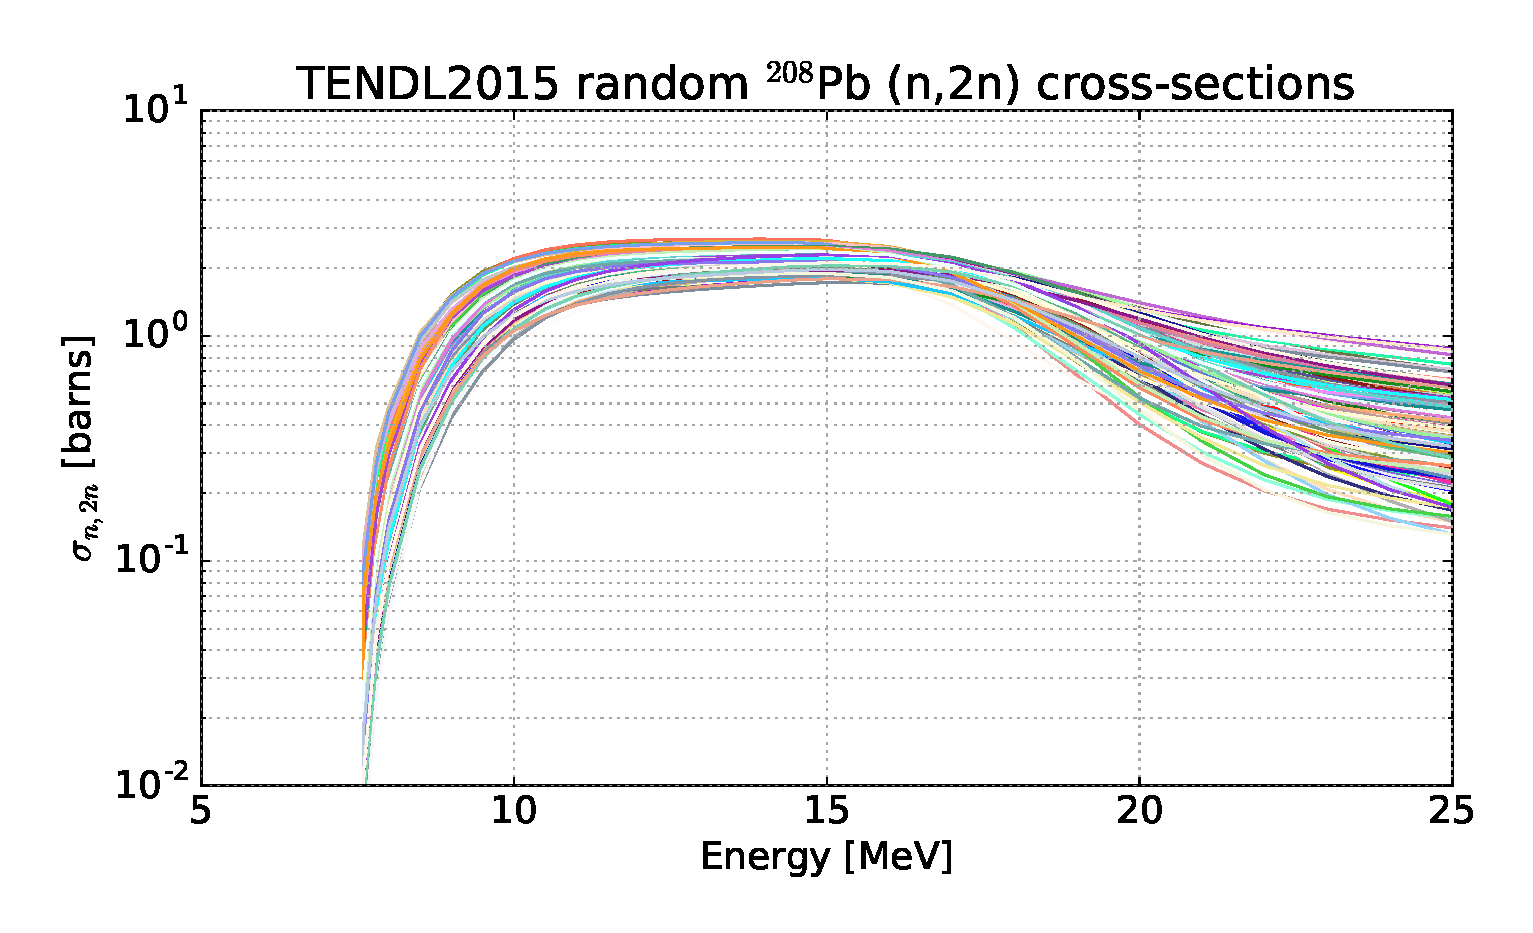
\includegraphics[width=0.48\textwidth]{pb208_tendl_n2n}
%   \caption{Shown here are 300 `random' TENDL2015 n,2n cross-sections as a function of energy for the most abundant lead isotope, $^{208}$Pb.}
%   \label{fig:tendl_lead}
% \end{figure}

\begin{figure}
%  \figuretitle{}
  \centering
  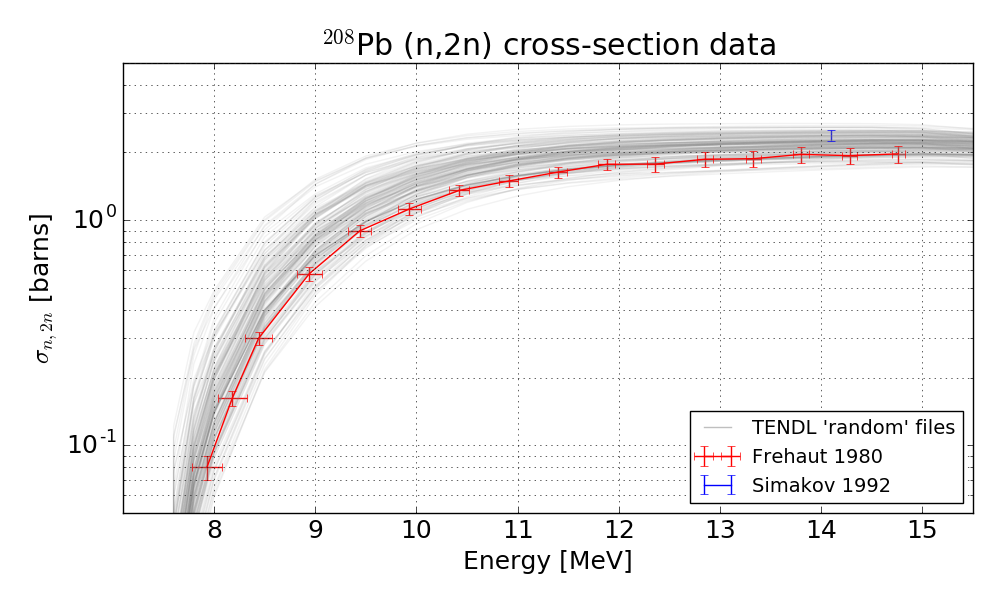
\includegraphics[width=\textwidth]{pb208_n2n_tendl_exfor.png}
  \caption{Shown here are $^{208}$Pb (n,2n) cross-sections as a function of energy. The plot shows the TENDL `random' data extracted from ACE files. Additionally, the few available experimental results in EXFOR are plotted for comparison.}
  \label{fig:tendl_lead}
\end{figure}

In an unmoderated fusion neutron spectrum the dominant reaction channels for Pb are neutron multiplication (n,2n) and elastic scattering, at approximately 2 and 3 barns respectively. The ENDF utility code Inter was used to extract cross-section values at a given energy from the ENDF files. The resulting distributions and correlations were plotted as figures \ref{fig:tendl_n2n}, \ref{fig:tendl_nel} \& \ref{fig:pb_el_n2n_corr}. Figures \ref{fig:tendl_n2n} and \ref{fig:tendl_nel} were examined for their first 3 statistical moments. 

\begin{table}[ht]
  \footnotesize
  \centering 
  \begin{tabular}{llll}
    \toprule
    Nuclide & Mean, $\mu$ [b] & RSD, $\frac{\sigma}{\mu}$ & Skewness \\
    \midrule
    Pb206 & 2.11 & 8.1\% & -0.065 \\
    Pb207 & 2.12 & 10.7\% & -0.868 \\
    Pb208 & 2.17 & 9.7\% & -0.120 \\
    \bottomrule
  \end{tabular}
  \caption{TENDL2015 `random' Pb n,2n neutron multiplicity channel cross-section distribution statistics}
  \label{table:n2n} % is used to refer this table in the text
\end{table}

Figure \ref{fig:tendl_n2n} and Table \ref{table:n2n} show the distributions of TENDL-2015 cross-sections for (n,2n) at 14MeV. Lower values for $\sigma_{n,2n}$ will reduce the neutron multiplication of the blanket and, other quantities being equal, result in a reduced total neutron flux and therefore a lower TBR.

\begin{figure}[ht]
%  \figuretitle{}
	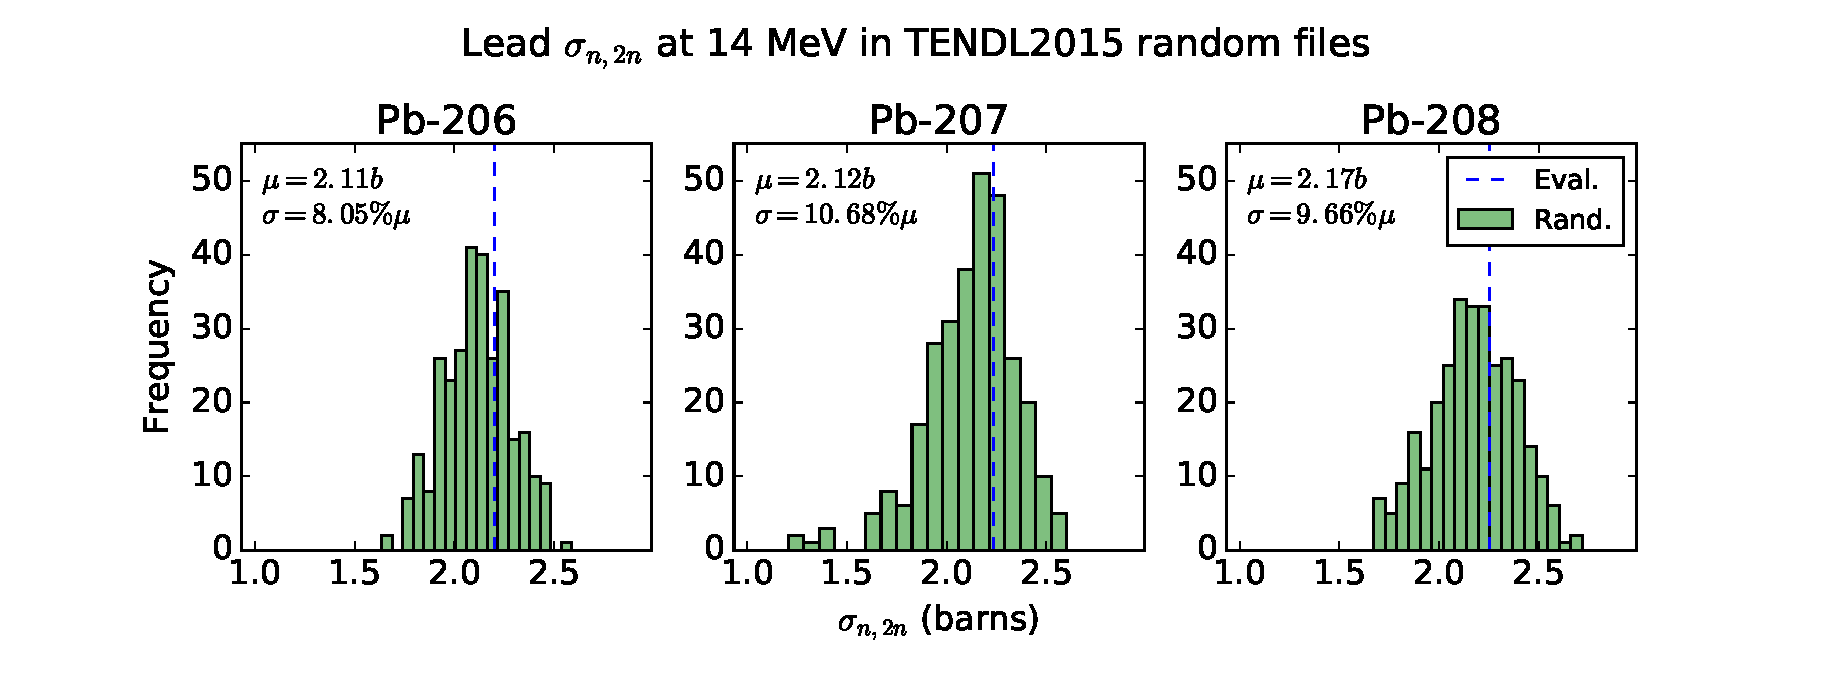
\includegraphics[width=\textwidth]{pb_tendl_n2n_hist}
	\caption{Shown are histograms of $\sigma_{n,2n}$ at 14MeV for the three major Pb isotopes. It can be seen that while $^{206,208}$Pb are approximately symmetrical with skewness values close to zero, $^{207}$Pb has a skewness of -0.868 indicating a low-value tail. This may or may not be representative of the underlying distribution. The histogram contains all 300 available files for $^{207}$Pb, but it could be the case that with more files a Gaussian shape would be recovered.}
	\label{fig:tendl_n2n}
\end{figure}

\begin{table}[ht]
  \footnotesize
  \centering 
  \begin{tabular}{llll}
    \toprule
    Nuclide & Mean, $\mu$ [b] & RSD, $\frac{\sigma}{\mu}$ & Skewness \\
    \midrule
    Pb206 & 2.84 & 7.5\% & 0.663 \\
    Pb207 & 2.80 & 8.0\% & 0.548 \\
    Pb208 & 2.81 & 8.1\% & 1.185 \\
    \bottomrule
  \end{tabular}
  \caption{TENDL2015 `random' Pb elastic scattering cross-section distribution statistics}
  \label{table:nel}
\end{table}

\begin{figure}[ht]
%  \figuretitle{}
  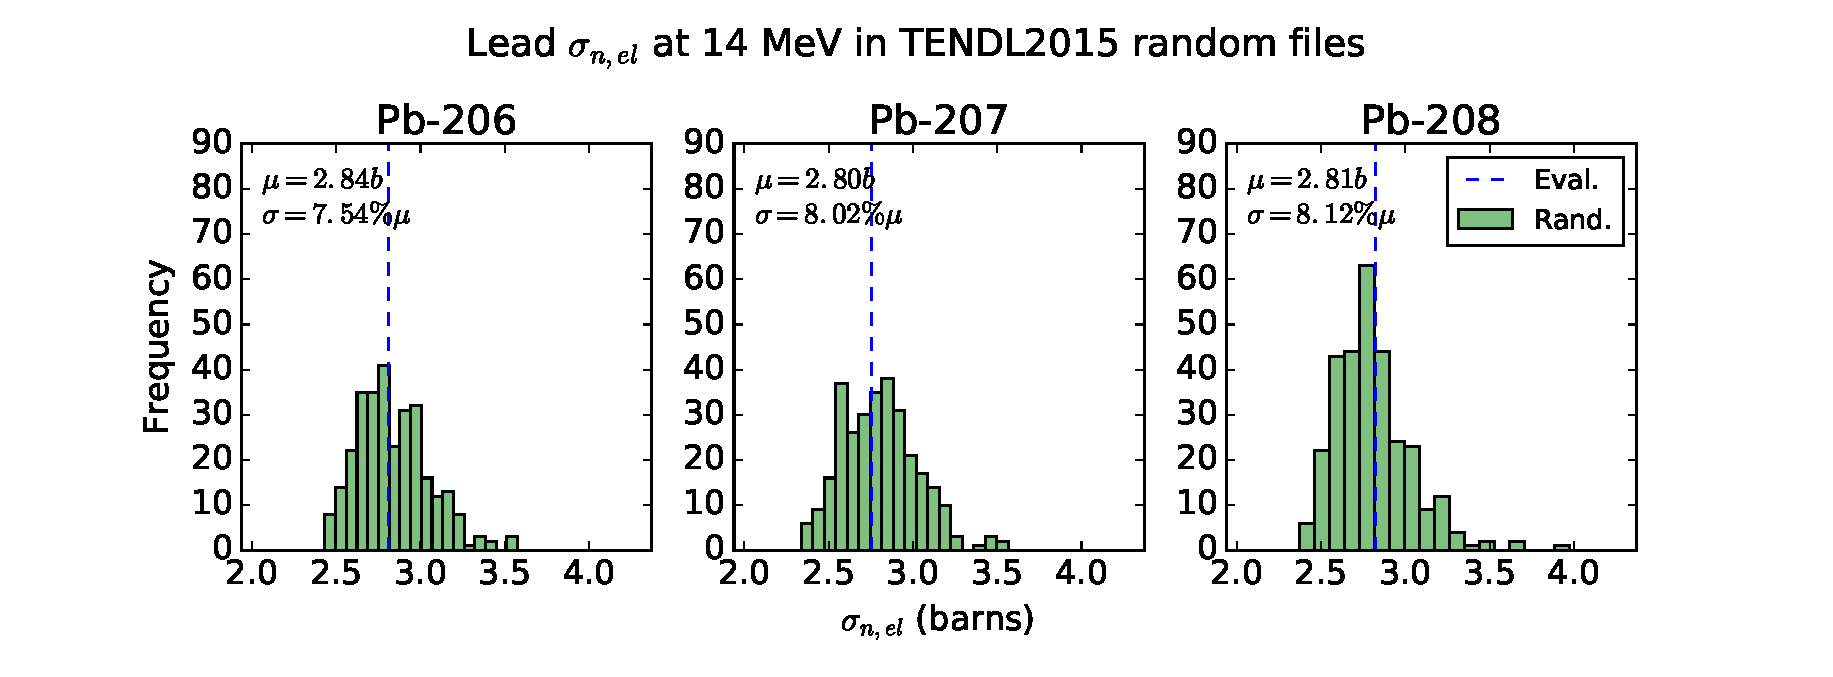
\includegraphics[width=\textwidth]{pb_tendl_nel_hist}
  \caption{The elastic scattering cross-sections for lead at 14MeV are all positively skewed, with $^{208}$Pb having a skewness value of 1.185.}
  \label{fig:tendl_nel}
\end{figure}

The elastic scattering data shown in Figure \ref{fig:tendl_nel} and Table \ref{table:nel} are instead positively skewed, with high value tails for each isotope, with the most pronounced tail being $^{208}$Pb. A greater elastic scattering cross-section will result in an increased likelihood of downscattering neutrons to lower energies. The softer spectrum will increase triton production in $^{6}$Li as the cross-section increases with decreasing energy, i.e. $\sigma_{n,t}(E) \propto \frac{1}{E}$. However, the elastic scattering cross-section is anti-correlated with the n,2n cross-section in the TENDL data (see figure \ref{fig:pb_el_n2n_corr}). In other words, a high scatter cross-section is typically coupled with a low multiplicity cross-section. This compensating effect decreases the overall uncertainty where individual perturbations on a single channel would result in an unrealistic, larger uncertainty. This inclusion of cross-channel correlation is one of the key advantages of TMC over more traditional uncertainty propagation (UP) methods. 

\begin{figure}[ht]
%  \figuretitle{}
	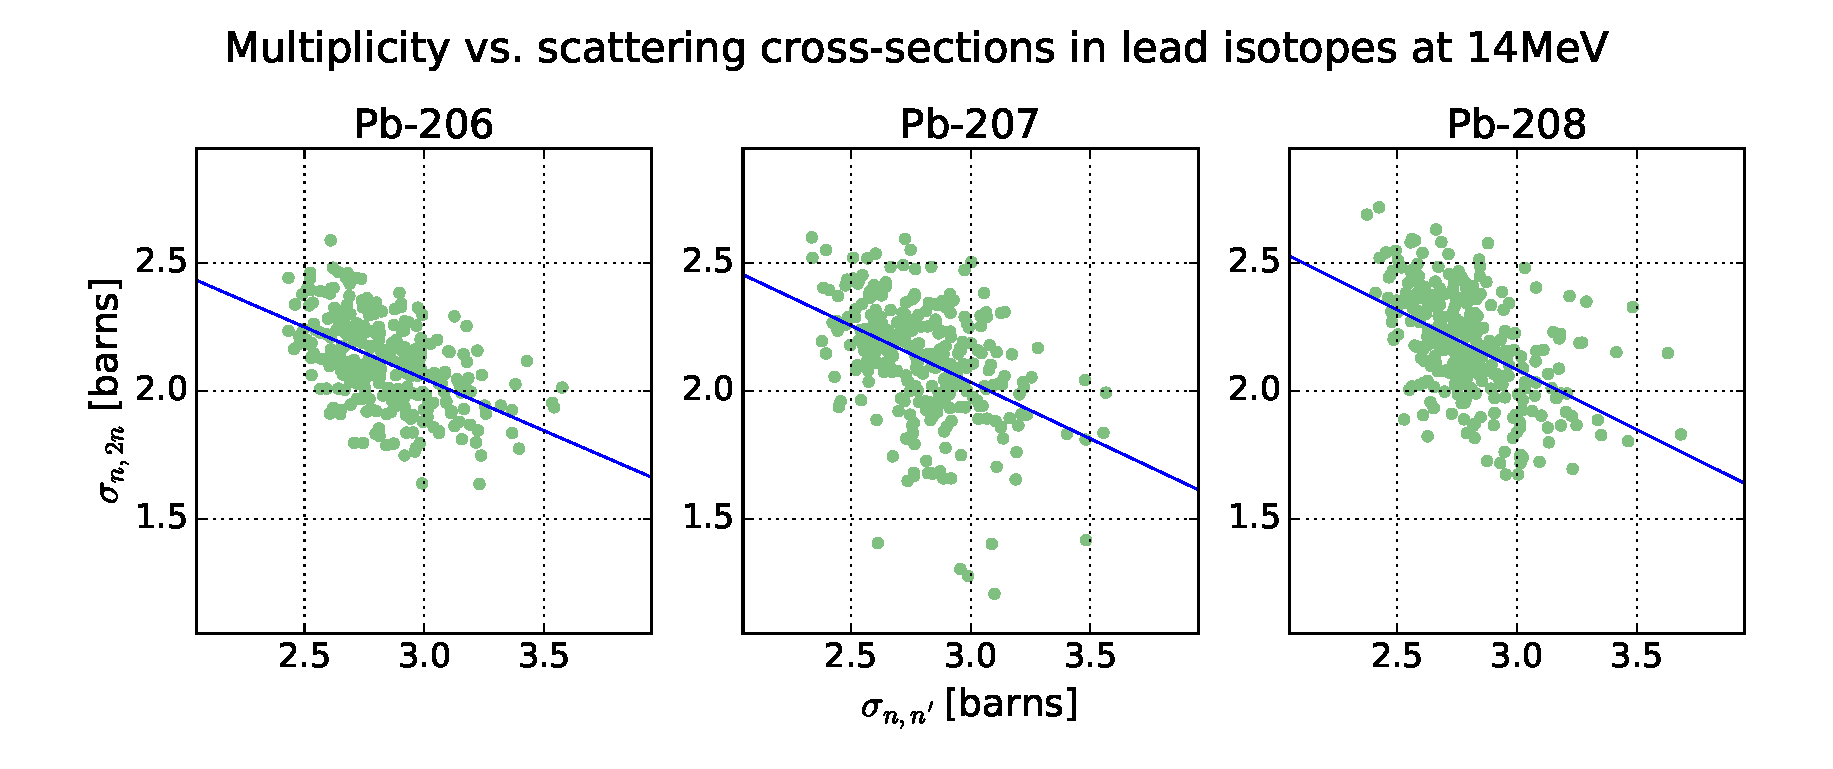
\includegraphics[width=\textwidth]{pb_el_n2n_corr}
  \caption{Shown here are scatter plots of the relationship between the scattering and n,2n cross-sections in the TENDL data. The two channels are clearly anti-correlated. A least squares fit has been applied and the resulting linear relationship plotted.}
	\label{fig:pb_el_n2n_corr}
\end{figure}

An 11.25\degree \ 2014 DEMO HCLL MCNP model was modified to tally TBR. The particle count was set to $3\cdot10^{6}$ giving a TBR relative standard deviation, RSD $\approx 0.002$ for each simulation. This is negligible compared to the total (nuclear data \& statistics) accumulated RSD and so the variance of the observable is assumed to be entirely due to variance in the nuclear data. While other TMC analyses have separated out the Monte-Carlo statistical variations to limit the computational cost \cite{Rochman2014a}, in this work the statistical variation has been strictly limited to avoid this issue. Whilst the Pb nuclear data employed was from TENDL-2015, FENDL3.1b data was used for the neutron transport of other elements present in the reactor model. A series of simple Bash and Python scripts were used to select different Pb TENDL-2015 ACE files for different runs, before creating and submitting jobs to the local cluster.

Python scripts were used to plot TBR convergence as a function of simulation count (see figure \ref{fig:convergence}) and the distributions of simulated TBR (see figure \ref{fig:tbr_distribution}).

\section{Results \& discussion}

The TMC simulation was run for a total of 1559 MCNP simulations, each 84 core-minutes across 32 cores. The total wall-clock time was 3 days, 15 hours.

\begin{figure}[ht]
%  \figuretitle{}
	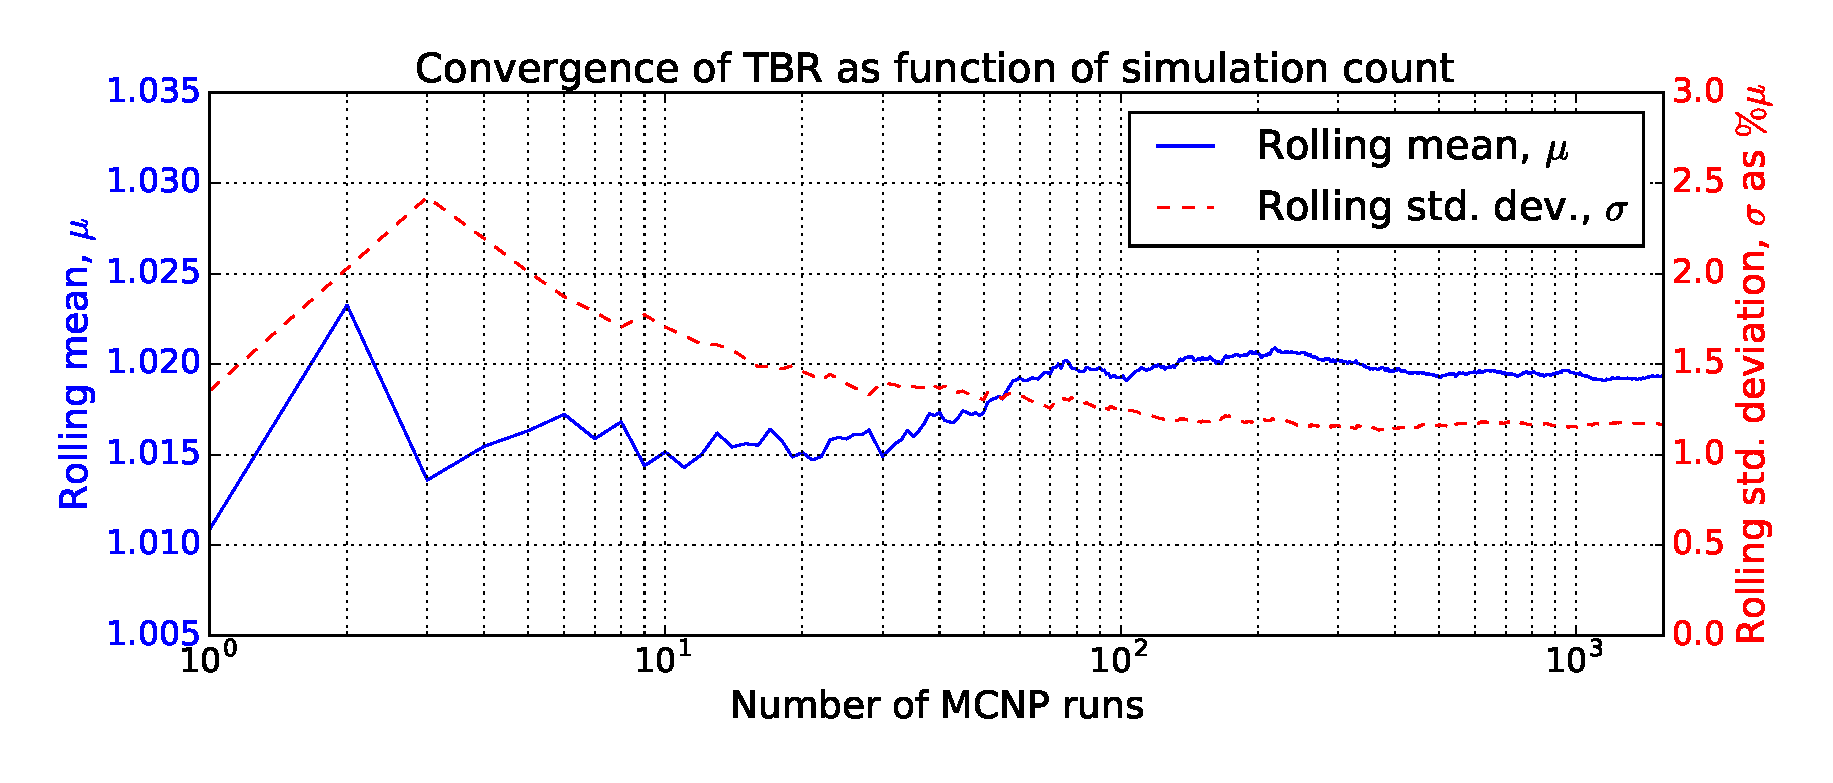
\includegraphics[width=\textwidth]{hcll_convergence_1559}
	\caption{The mean and standard deviation of the TBR distribution is presented as a function of the number of simulations. The TMC simulation can be seen to converge at approximately 400 MCNP runs. $\mu(400) \approx 1.02$ and $\sigma(400) \approx 1.14$.}
	\label{fig:convergence}
\end{figure}

The mean TBR value is 1.0193 whilst the median is 1.0200, with a one sigma standard deviation of 0.012 or 1.2\% of the mean. The TBR distribution is approximately normal, with a small skewness of -0.199, meaning the low-value TBR tail is longer than the high-value tail. Figure \ref{fig:tbr_n2n} shows the expected correlation between the n,2n cross-sections used in a given simulation and the TBR attained in that simulation.

\begin{figure}[ht]
%  \figuretitle{}
  \centering
	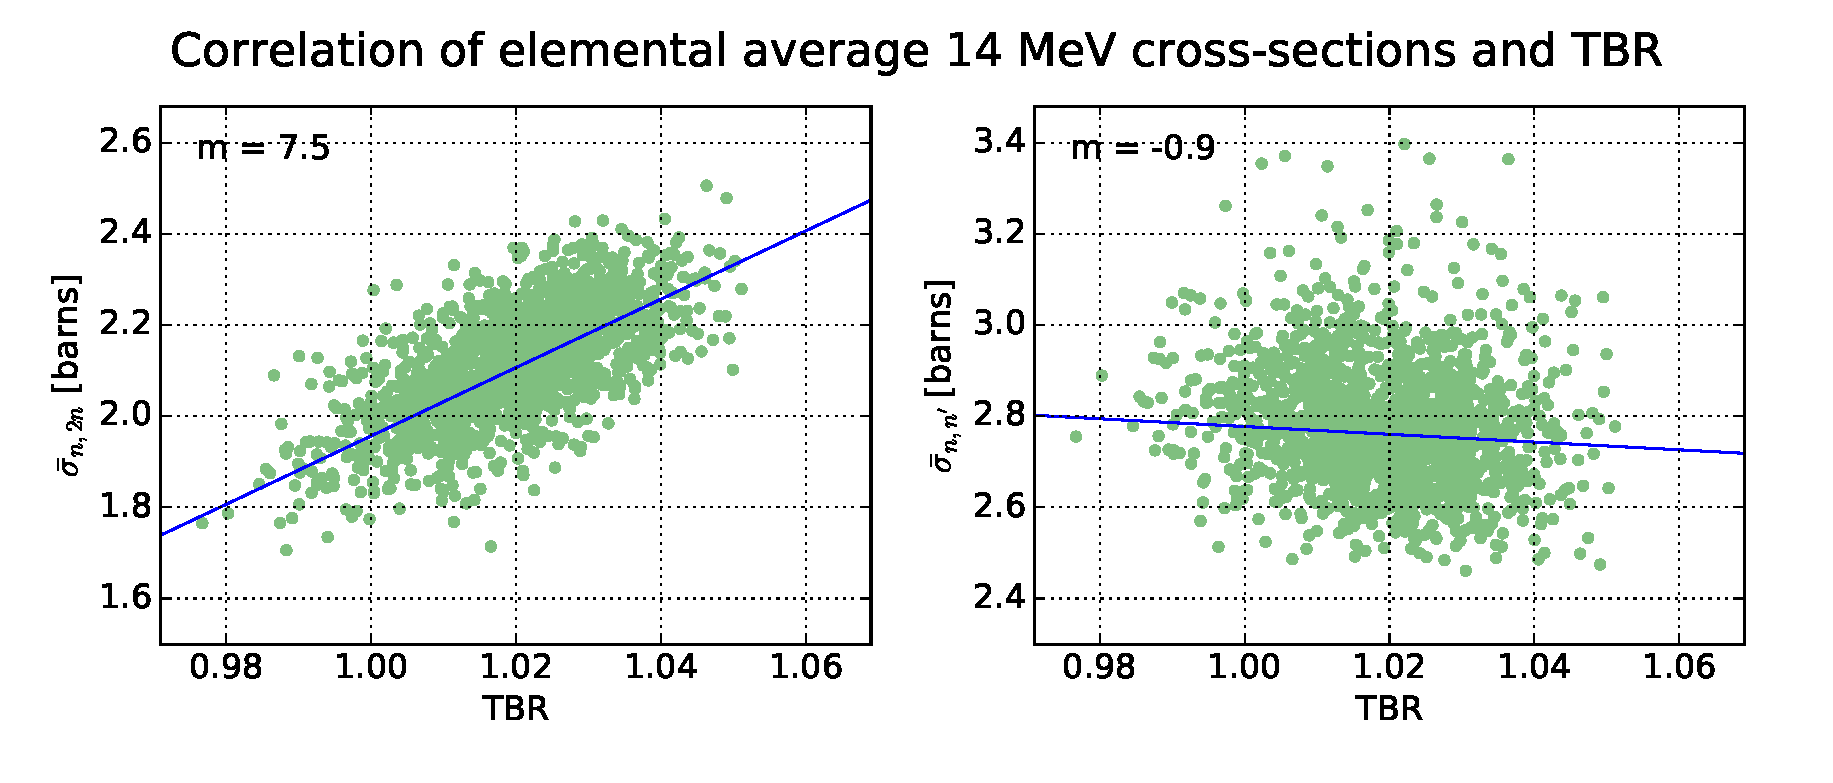
\includegraphics[width=\textwidth]{pb_tbr_n2n_el_corr}
	\caption{Above are scatter plots of average cross-sections for the n,2n (left) and elastic (right) channels against resulting TBR value. As the cross-sections for each of the three lead isotopes were varied in every simulation, so the cross-sections plotted here are the elemental average values denoted as $\bar{\sigma}_{n,2n}$ or $\bar{\sigma}_{n,n'}$, i.e. all three varied Pb isotopes contribute, weighted by their relative natural abundances. The n,2n cross-section is positively correlated with the TBR value as expected. There is less of a relationship between scattering and TBR.}
	\label{fig:tbr_n2n}
\end{figure}

Uncertainty propagation in Monte-Carlo type radiation transport problems has often previously been computed using linear perturbation theory approaches. Unfortunately these are only applicable for small changes in the input data. They are also unable to reproduce probability distributions of the integral quantity of interest \cite{Rising2012}. Whilst figure \ref{fig:tbr_distribution} shows a TBR distribution that is not tremendously skewed, that is not to say other fusion quantities will not be. Koning \& Rochman have demonstrated that fast and accelerator driven fission systems can have significantly skewed k$_{\mbox{eff}}$ values, best described by an Extreme Value Fit (EVD) \cite{Koning2008}.

\begin{figure}
%  \figuretitle{}
	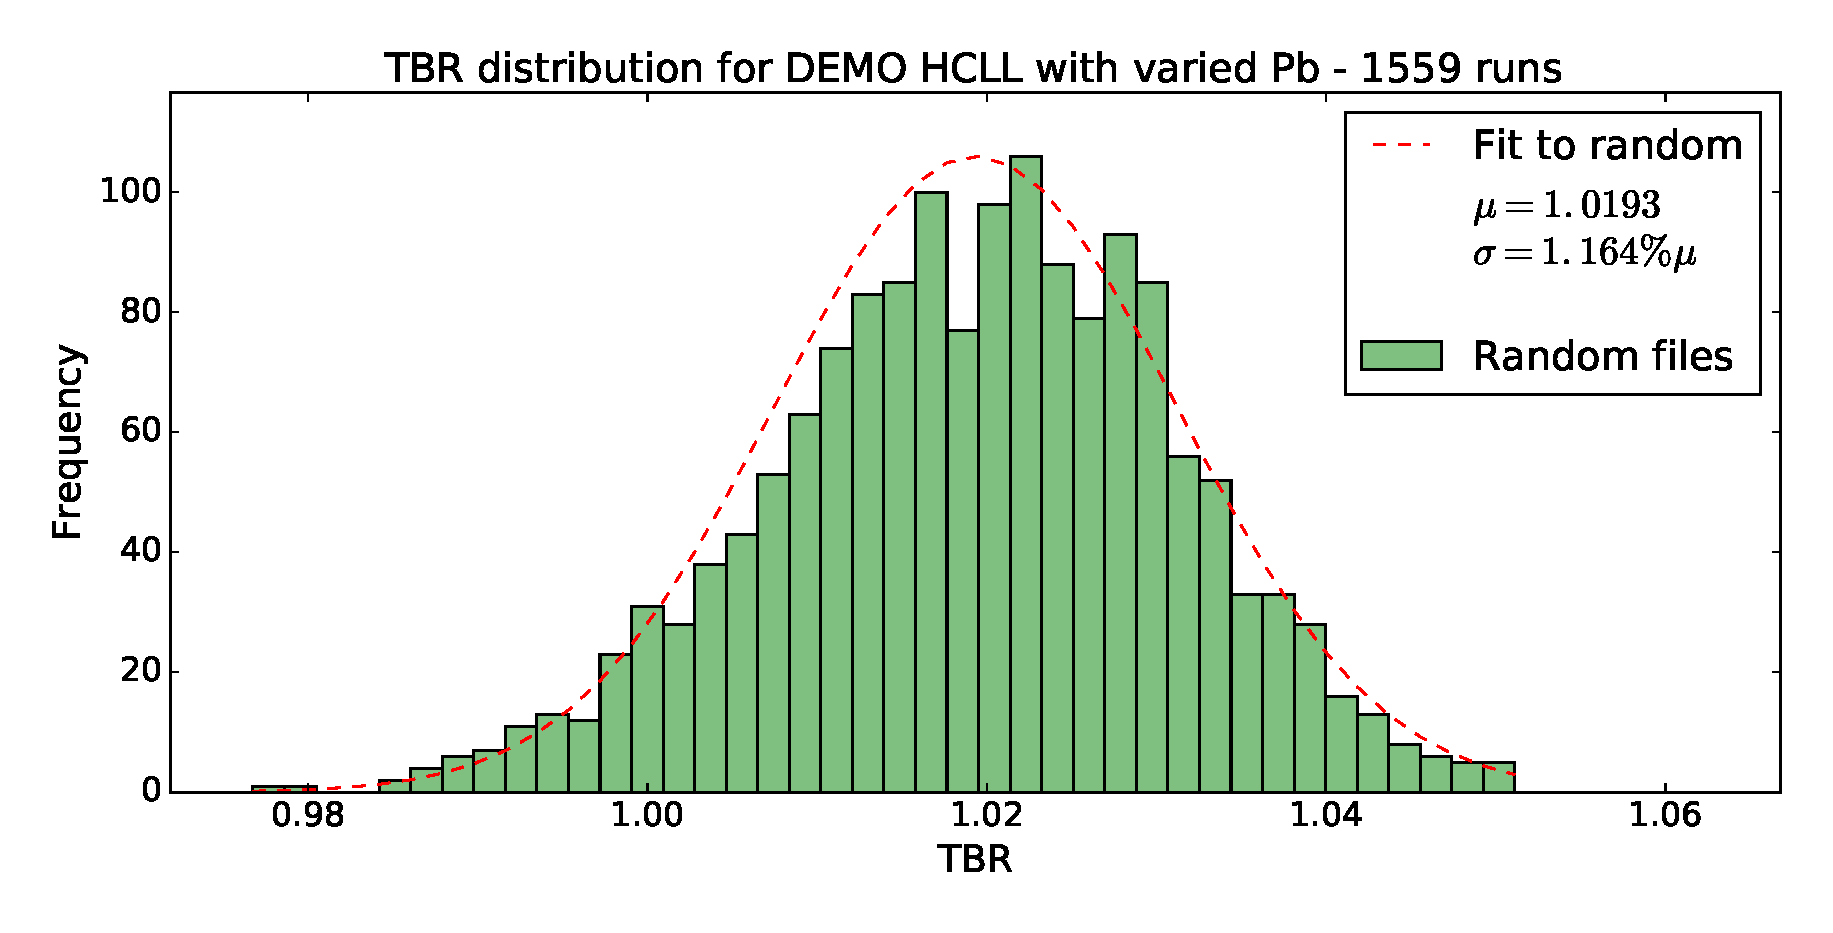
\includegraphics[width=\textwidth]{hcll_hist_1559}
	\caption{Histogram of TBR values computed with the TMC methodology.}
	\label{fig:tbr_distribution}
\end{figure}

\section{Conclusion}
TBR uncertainty has been computed with the TMC technique, investigating the contribution of uncertain nuclear data from the three major lead isotopes. The standard deviation is 1.2\% of the mean TBR. However, note that 5.8\% of the distribution is less than unity. While the average value may appear to be feasible, it should be stressed that there is a non-negligible probability of a value below a required limit. The TBR values are relatively low as this particular model has not been optimised for TBR and any practical design should have a TBR $\approx 1.1$ \cite{Fischer2015}, but in future design studies engineers should be aware of the probability of non-compliant operational parameters. 

The TENDL-2015 nuclear data investigated in section \ref{sec:data}, which is not necessarily Gaussian in shape, has yielded a TBR distribution with a small but finite negative skewness, an extended low-value tail. It is not possible to deduce this shape with more simplified approaches to uncertainty propagation such as linear perturbation theory.

Future work on TBR in HCLL could include the effect of other nuclides and elements which TBR is sensitive to including iron, as well as a completely correlated uncertainty propagation method employing lithium. 

More generally, when solving for integral quantities in nuclear fusion systems, thought should be given to fully-correlated uncertainty propagation and the form of the resulting probability distributions. In particular, whether a non-normal distribution with increased likelihood of extreme behaviour would have engineering design or safety implications for TBR, nuclear heating, fast flux, gas production or damage terms. Moreover, in all analyses for design applications the non-negligible probability of operational parameters in unacceptable regimes should be borne in mind.

